\section{Architettura del prodotto}\label{section:architettura del prodotto}
%Descrizione pattern architetturale 
\subsection{Descrizione generale}
Il pattern architetturale scelto dal gruppo per lo sviluppo del progetto è il Model-View-ViewModel. Il
seguente pattern è tra i più diffusi nello sviluppo delle web application e permette di scrivere codice
facilmente mantenibile e riusabile; questo è possibile grazie al forte disaccoppiamento che sussiste tra
logica di presentazione e di business. Inoltre l'MVVM è risultato il più adatto per essere utilizzato con
React, libreria impiegata per lo sviluppo dell'UI e che renderizza le componenti in base al loro stato
interno.
\begin{itemize}
\item Model: questa porzione ricopre la logica di business dell'applicazione; %da aggiungere 
\item ViewModel: qui viene effettuato il binding tra View e Model ed è contenuta la loro logica;
\item View: questa porzione gestisce la presentazione tramite una specifica gerarchia di componenti;
ciascun componente contiene la logica strettamente legata alla sua visualizzazione e necessaria al
mantenimento del proprio stato interno.
\end{itemize}

Il passaggio dei dati dal Model alle varie componenti grafiche avviene attraverso l'utilizzo di un Context
React, al quale viene passato un'istanza del ViewModel. L'utilizzo di un Context React ci permette di
accedere al valore corrente del ViewModel in qualsiasi porzione della View, senza doverlo passare di
componente in componente attraverso le props (ossia gli argomenti dei componenti che compongono la
vista). Nella radice dell'applicazione viene infatti creata un'istanza del ViewModel, che viene passata
ad un Context.Provider, che fa da contenitore per tutta la View. All'interno di tale contenitore ogni
componente può utilizzare un hook per accedere al Context React ed utilizzare il valore più recente del ViewModel.

È stato scelto di utilizzare un Context React per il passaggio dei dati in quanto la nostra applicazione è
molto profonda e non risultava conveniente passare i dati per molti componenti rischiando, nel peggiore
dei casi, di doverli utilizzare nell'ultimo della gerarchia.
Per poter fare in modo che una componente della View si renderizzi non solo al cambiamento del
suo stato interno ma anche al cambiamento dei dati nel Model, abbiamo utilizzato la libreria Mobx.
Questa ci permette di implementare l'observer pattern, non supportato di default da React. A tale
scopo, Mobx permette di segnare delle classi (o attributi di esse) come "observable" e di costruire
dei componenti della View come "observer". Quest'ultimi vengono automaticamente ri-renderizzati al
cambiamento di un qualsiasi attributo observable.

\subsection{Diagramma delle classi}

In questa sezione verrà mostrato il diagramma delle classi dell'applicazione, 
per una maggiore fruibilità i diagrammi della parte frontend sono stati divisi in quattro parti.
Le classi colorate compaiono più volte nei vari diagrammi.

\begin{figure}[H]
    \begin{center}
    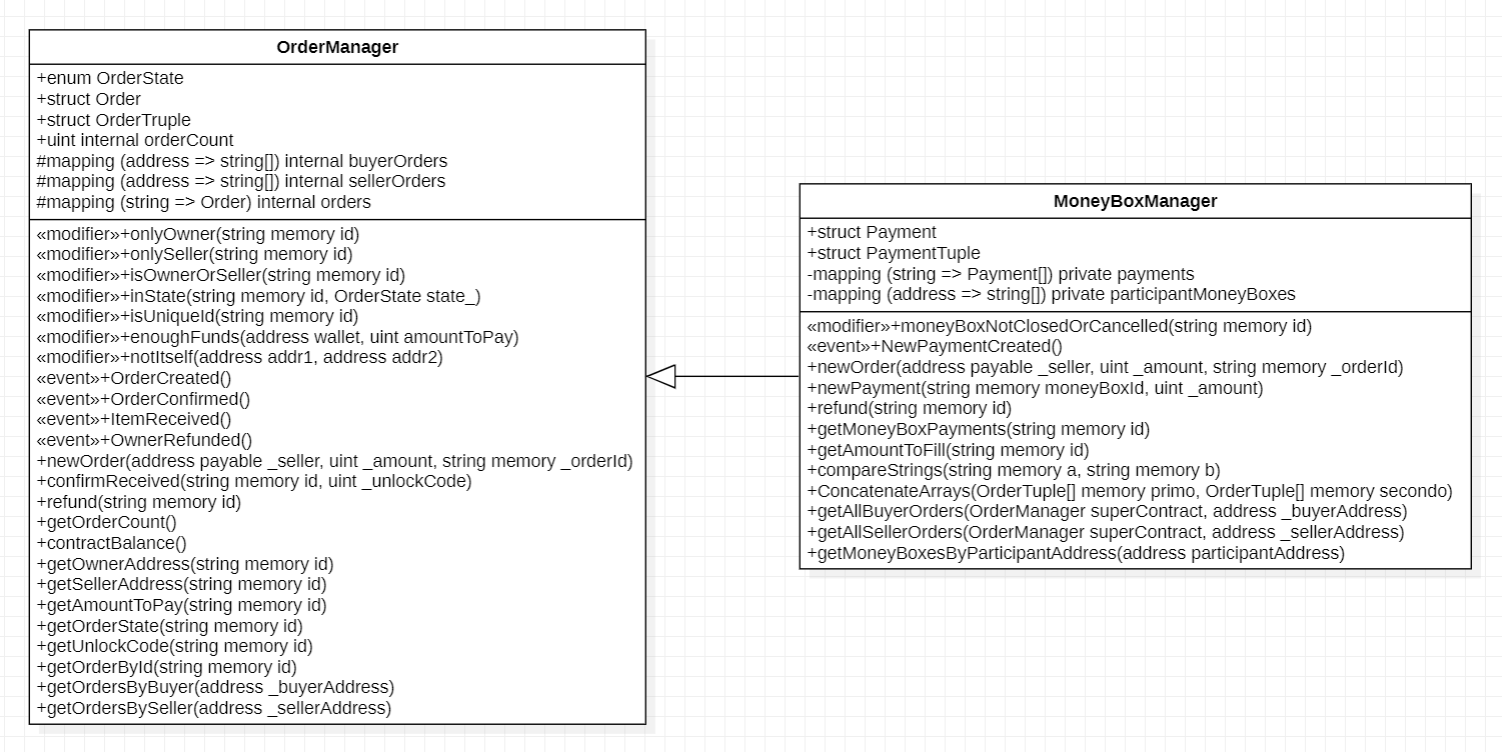
\includegraphics[scale=0.5]{immagini/smartcontracts.png}
    \caption{Classi Solidity}
    \end{center}
\end{figure}

\begin{landscape}
\begin{figure}[H]
    \begin{center}
    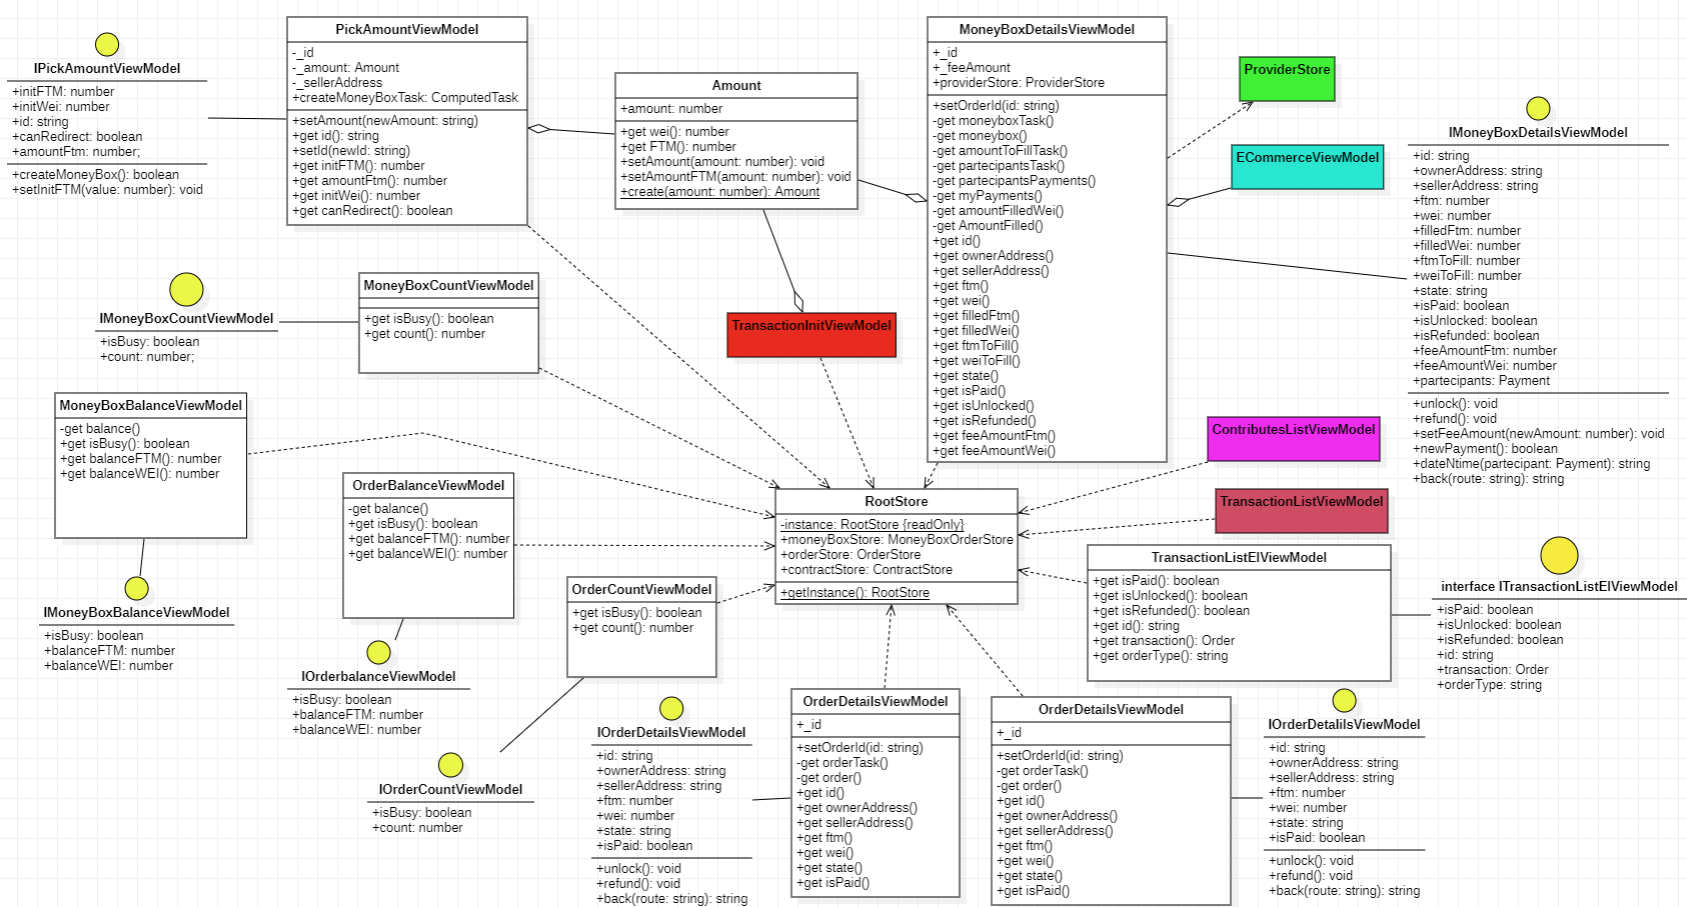
\includegraphics[scale=0.7]{immagini/rootstore.png}
    \caption{RootStore e classi correlate}
    \end{center}
\end{figure}
\end{landscape}

\begin{landscape}
    \begin{figure}[H]
        \begin{center}
        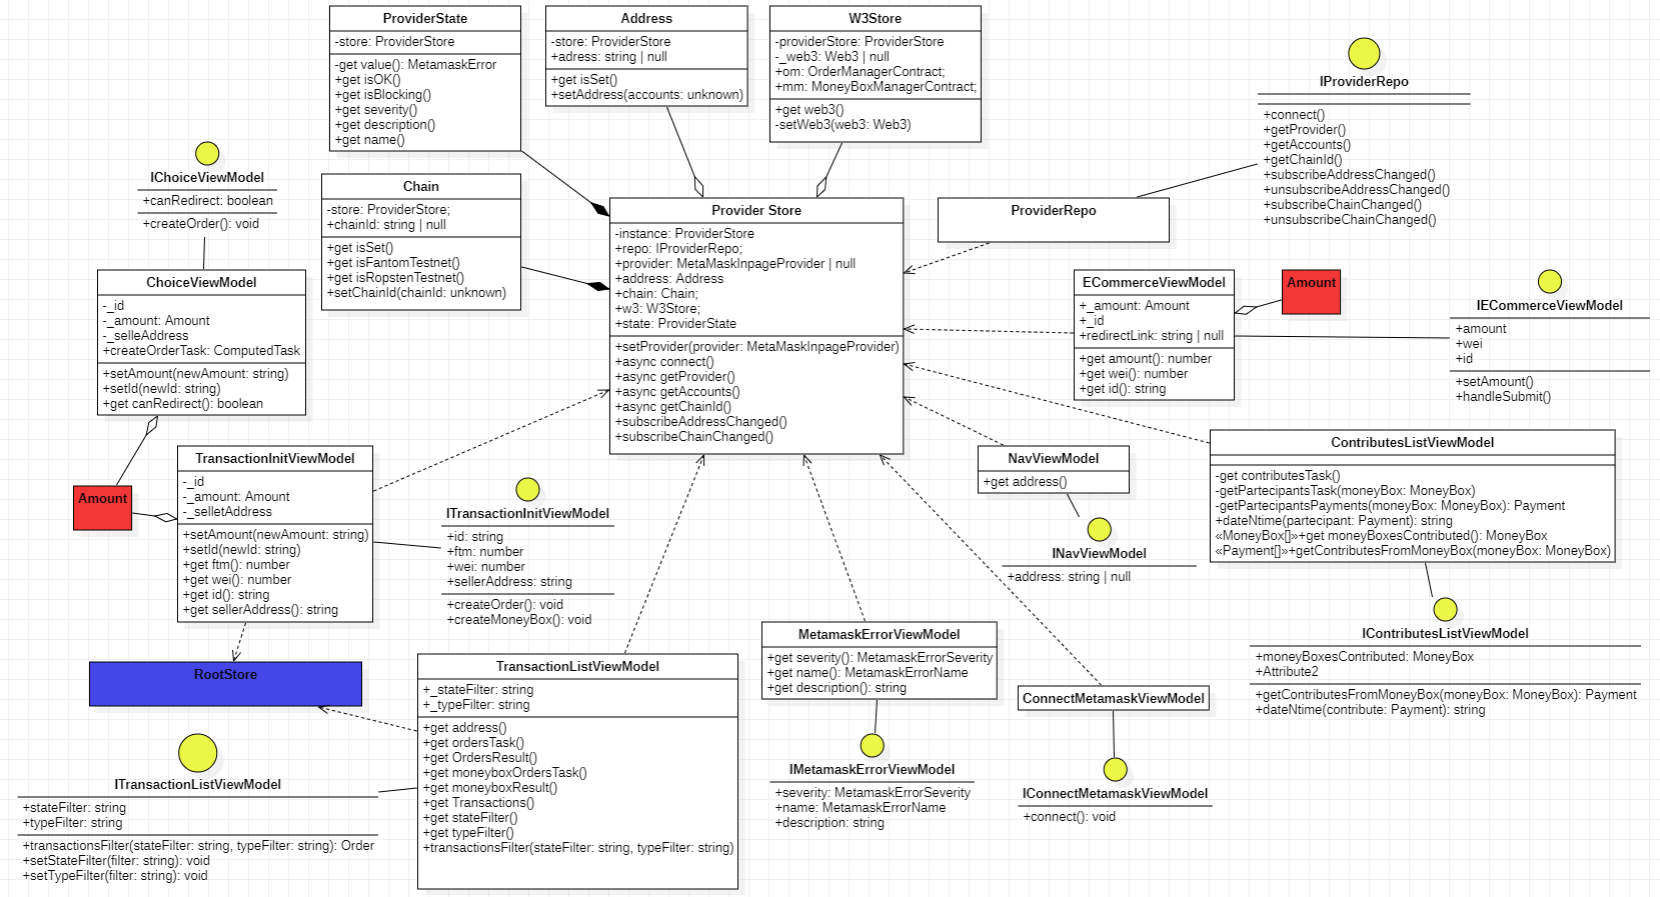
\includegraphics[scale=0.7]{immagini/providerstore.png}
        \caption{ProviderStore e classi correlate}
        \end{center}
    \end{figure}
\end{landscape}

\begin{landscape}
    \begin{figure}[H]
        \begin{center}
        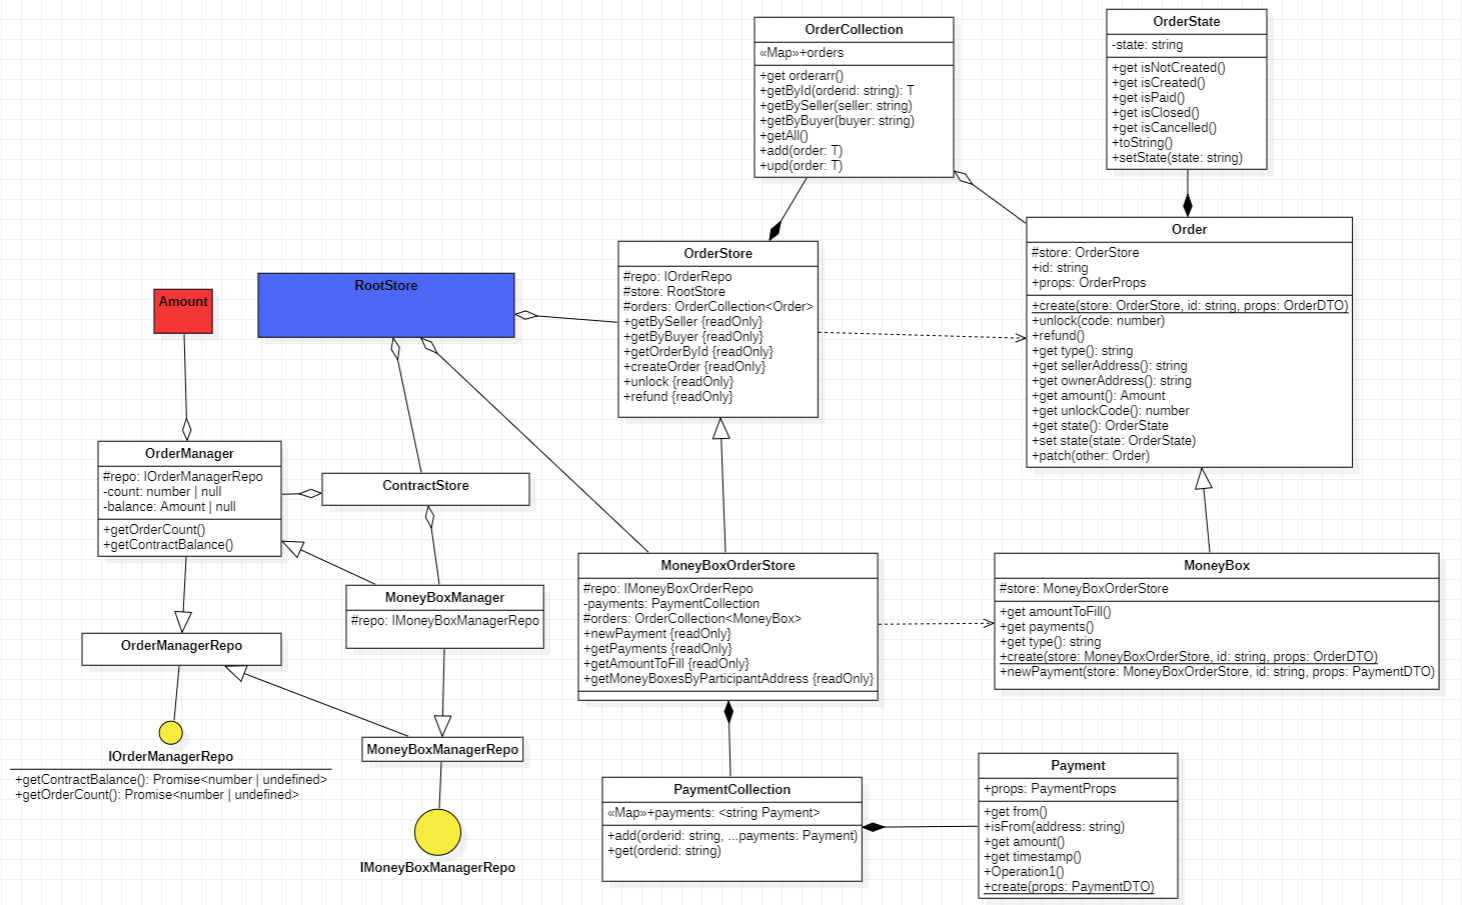
\includegraphics[scale=0.7]{immagini/order_moneybox.png}
        \caption{Gerarchia Order e MoneyBox}
        \end{center}
    \end{figure}
\end{landscape}

\begin{landscape}
    \begin{figure}[H]
        \begin{center}
        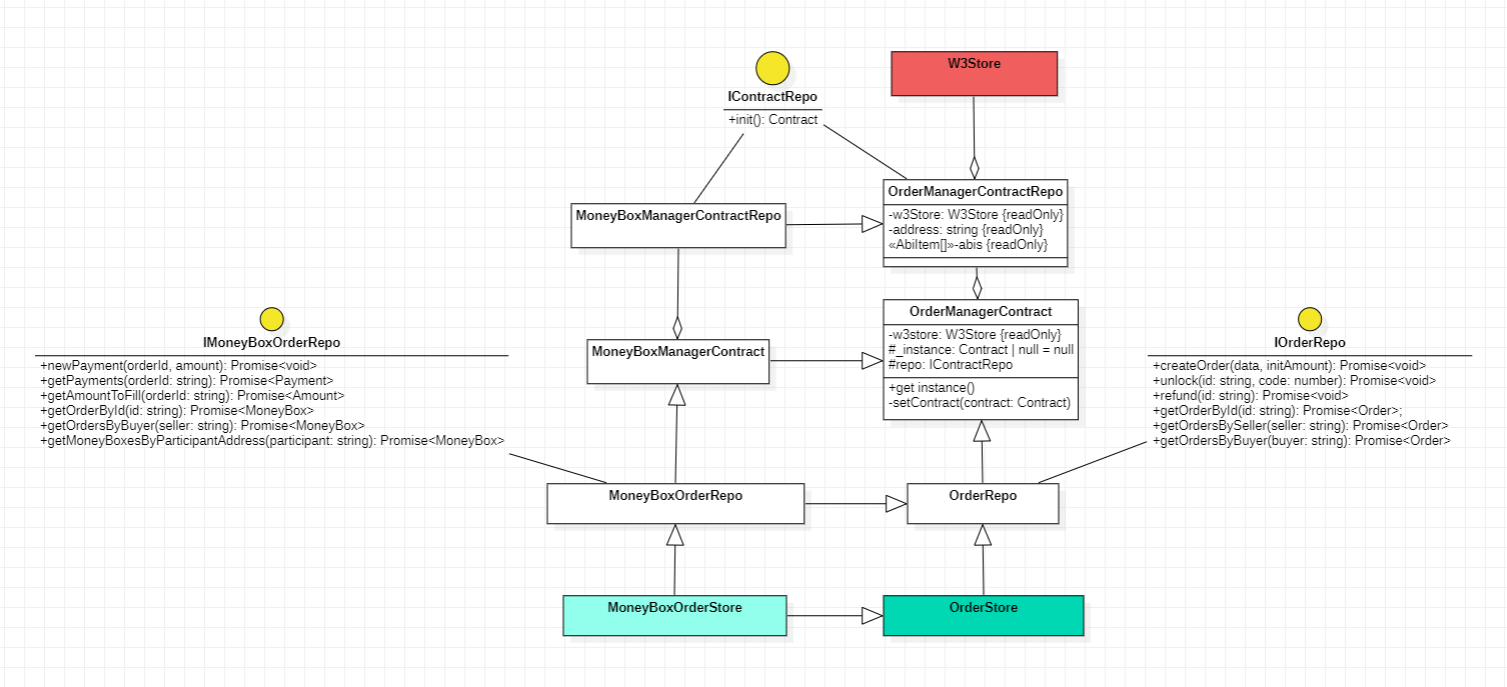
\includegraphics[scale=0.7]{immagini/contractrepo.png}
        \caption{Passaggio da Web3Store a OrderStore}
        \end{center}
    \end{figure}
\end{landscape}
    
\subsection{Diagrammi di sequenza}

Vengono di seguito riportati i diagrammi di sequenza per le operazioni più importanti dell'applicazione.

\begin{figure}[H]
    \begin{center}
    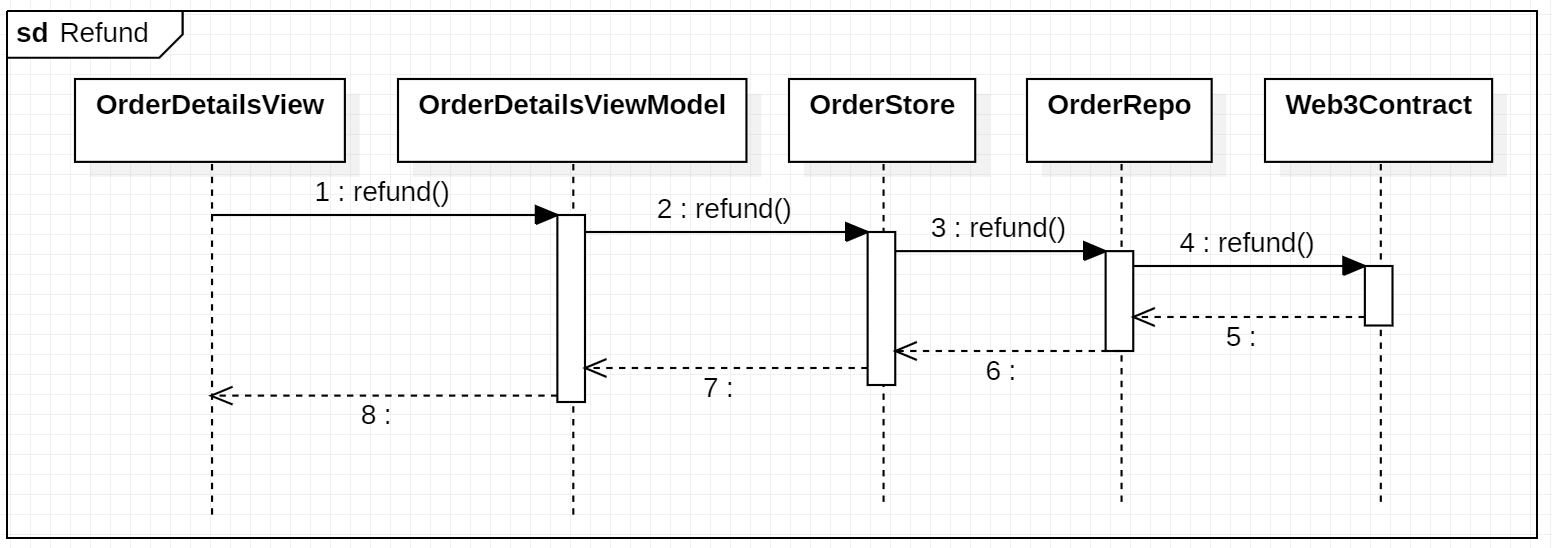
\includegraphics[width=\textwidth]{immagini/refund.png}
    \caption{Diagramma di sequenza della funzione di Refund}
    \end{center}
\end{figure}

\begin{figure}[H]
    \begin{center}
    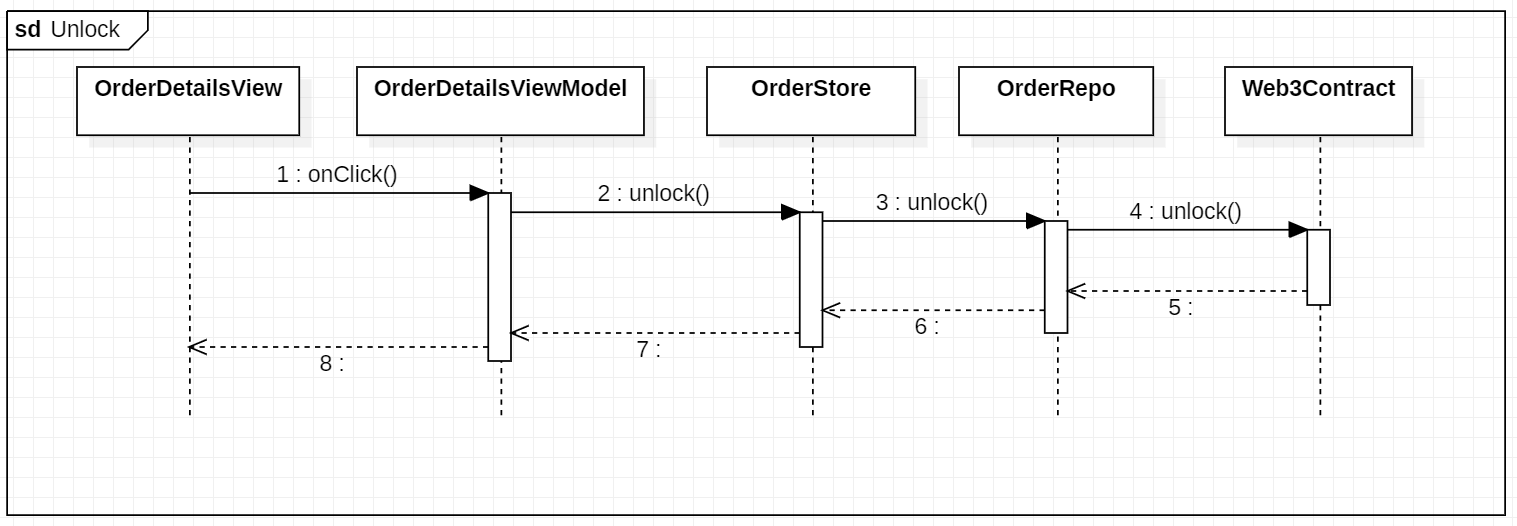
\includegraphics[width=\textwidth]{immagini/unlock.png}
    \caption{Diagramma di sequenza della funzione di Unlock}
    \end{center}
\end{figure}

\begin{landscape}
    \begin{figure}[H]
        \begin{center}
        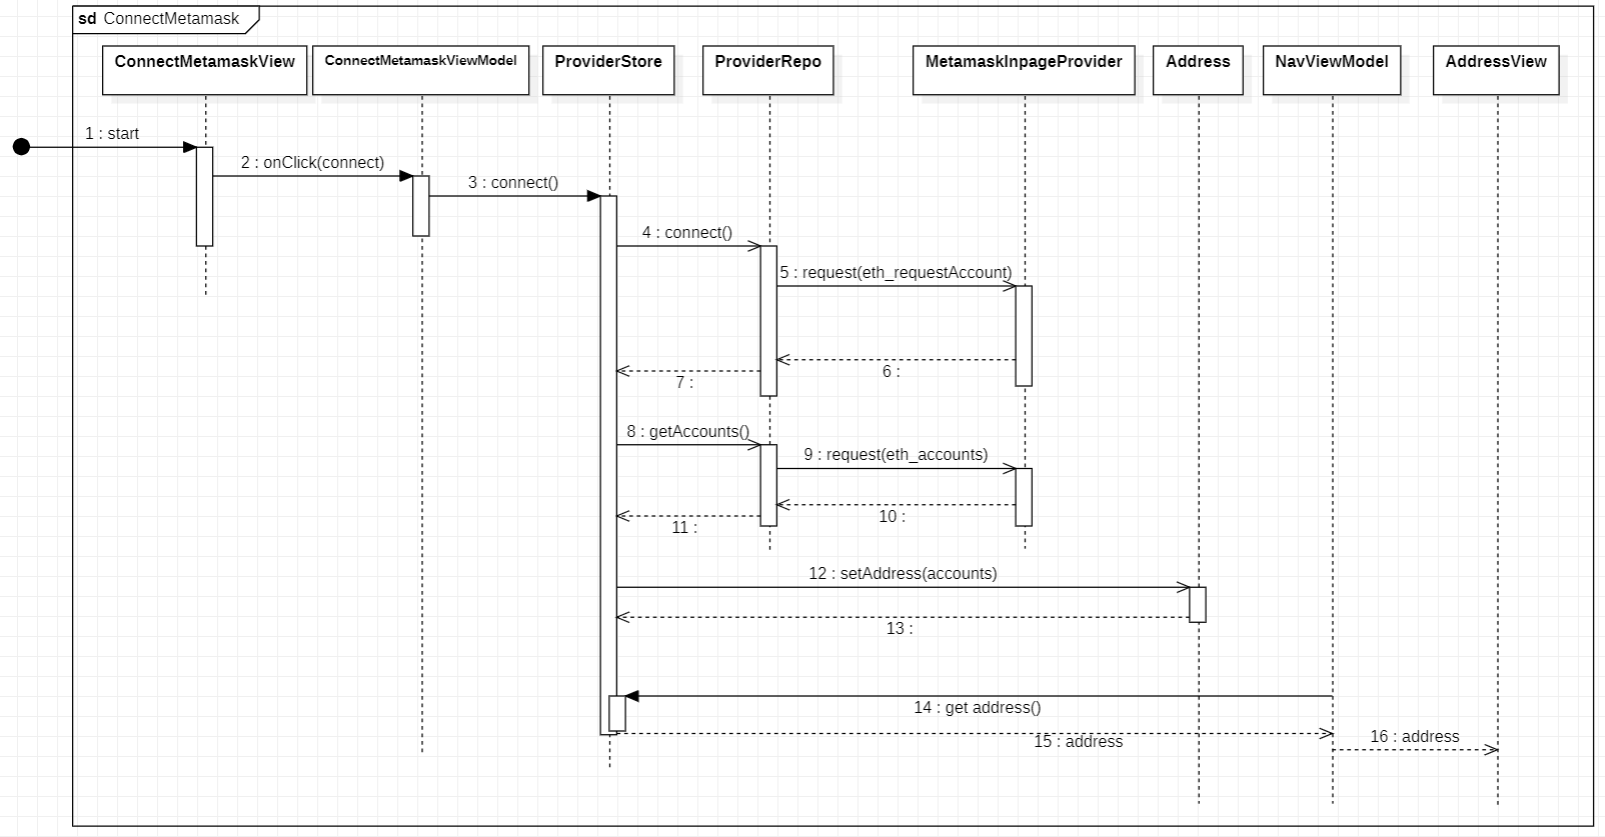
\includegraphics[scale=0.7]{immagini/connect_metamask.png}
        \caption{Diagramma di sequenza della funzione di connessione a Metamask}
        \end{center}
    \end{figure}
\end{landscape}

\begin{landscape}
    \begin{figure}[H]
        \begin{center}
        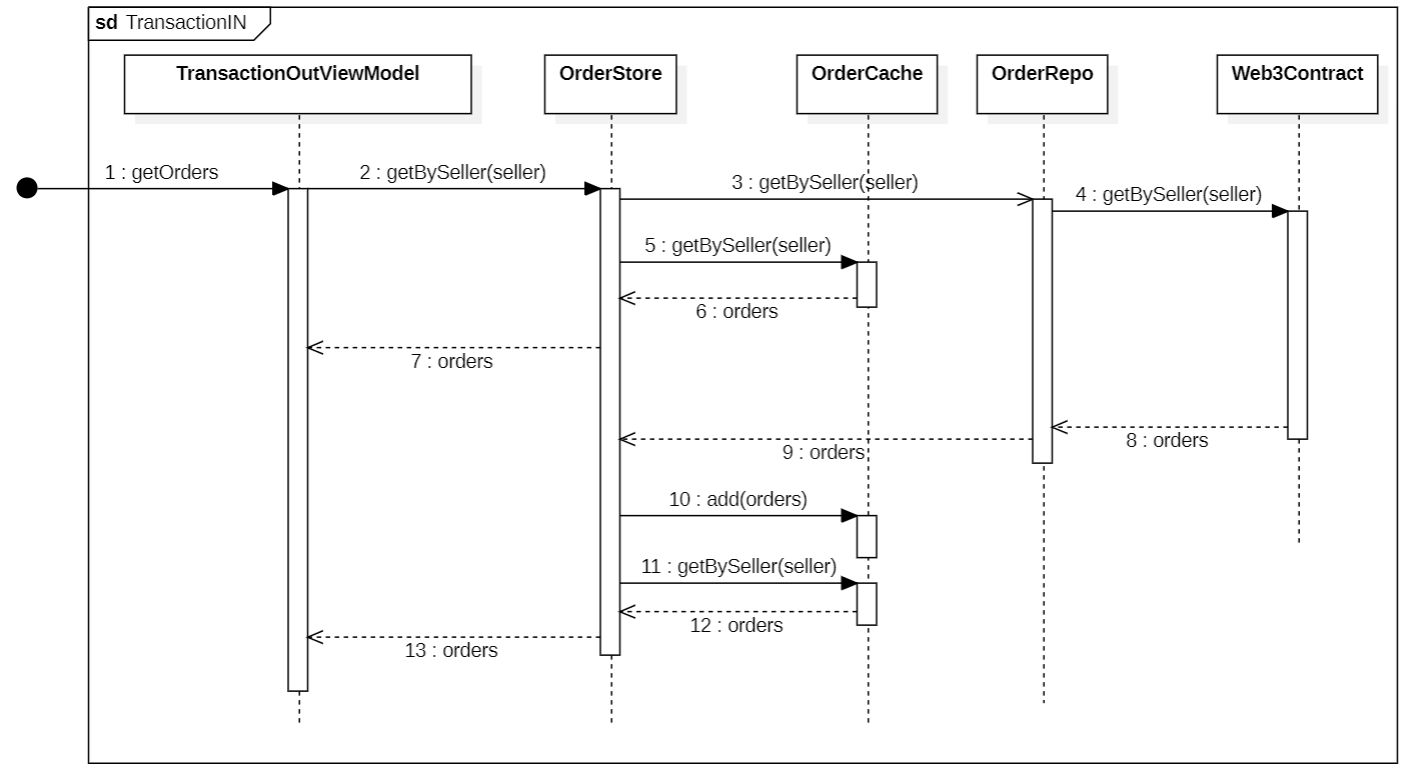
\includegraphics[scale=0.7]{immagini/TransactionIn.png}
        \caption{Diagramma di sequenza della selezione delle transazioni in entrata}
        \end{center}
    \end{figure}
\end{landscape}

\begin{landscape}
    \begin{figure}[H]
        \begin{center}
        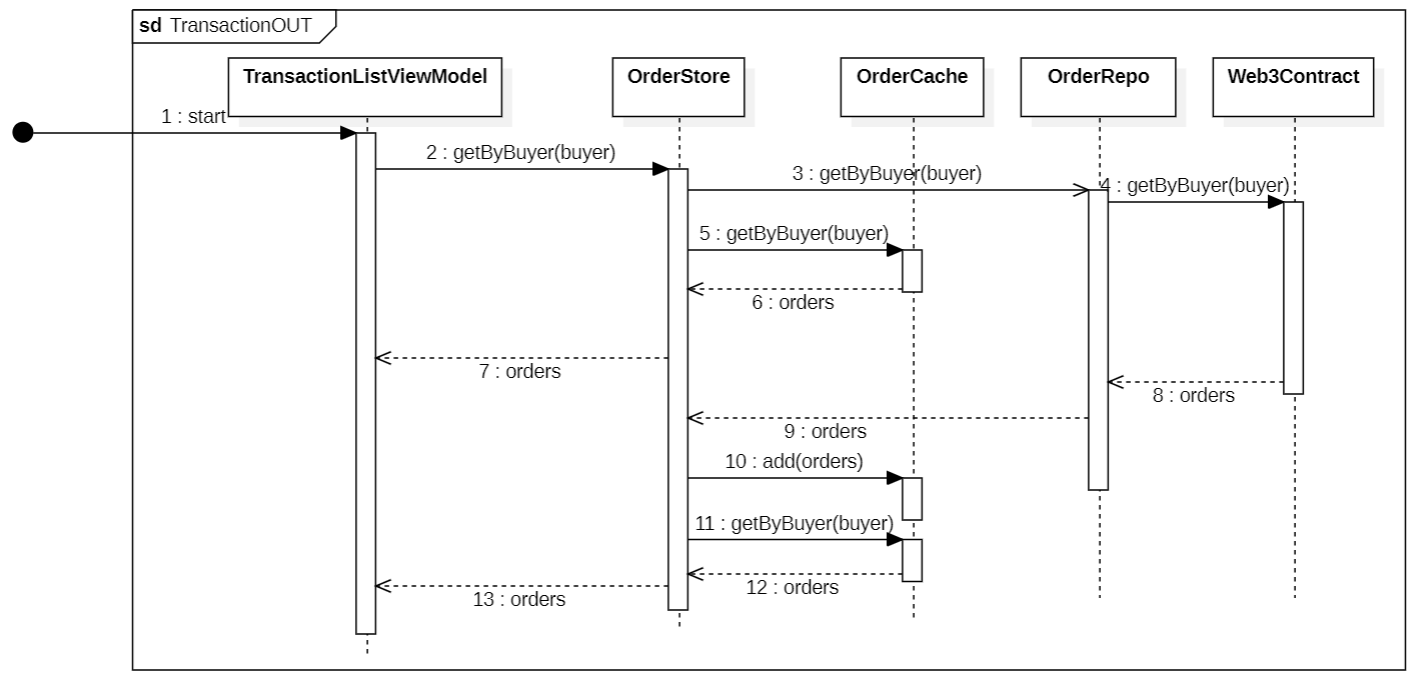
\includegraphics[scale=0.7]{immagini/TransactionOut.png}
        \caption{Diagramma di sequenza della selezione delle transazioni in uscita}
        \end{center}
    \end{figure}
\end{landscape}

\begin{figure}[H]
    \begin{center}
    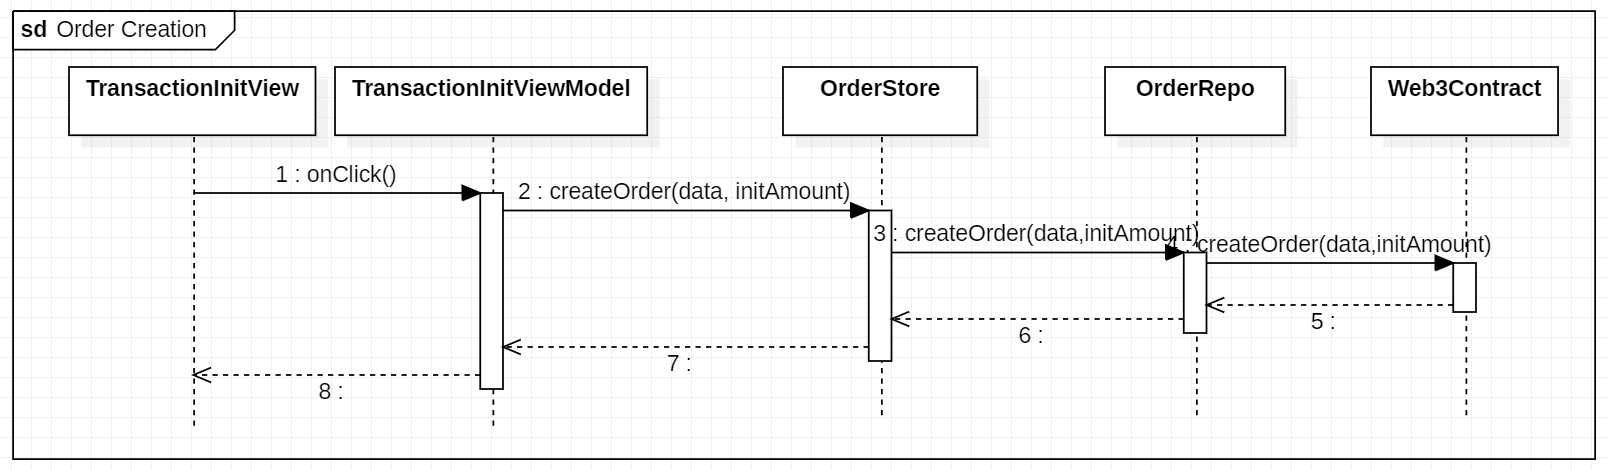
\includegraphics[width=\textwidth]{immagini/ordercreation.png}
    \caption{Diagramma di sequenza della funzione di creazione di un nuovo ordine}
    \end{center}
\end{figure}

\begin{figure}[H]
    \begin{center}
    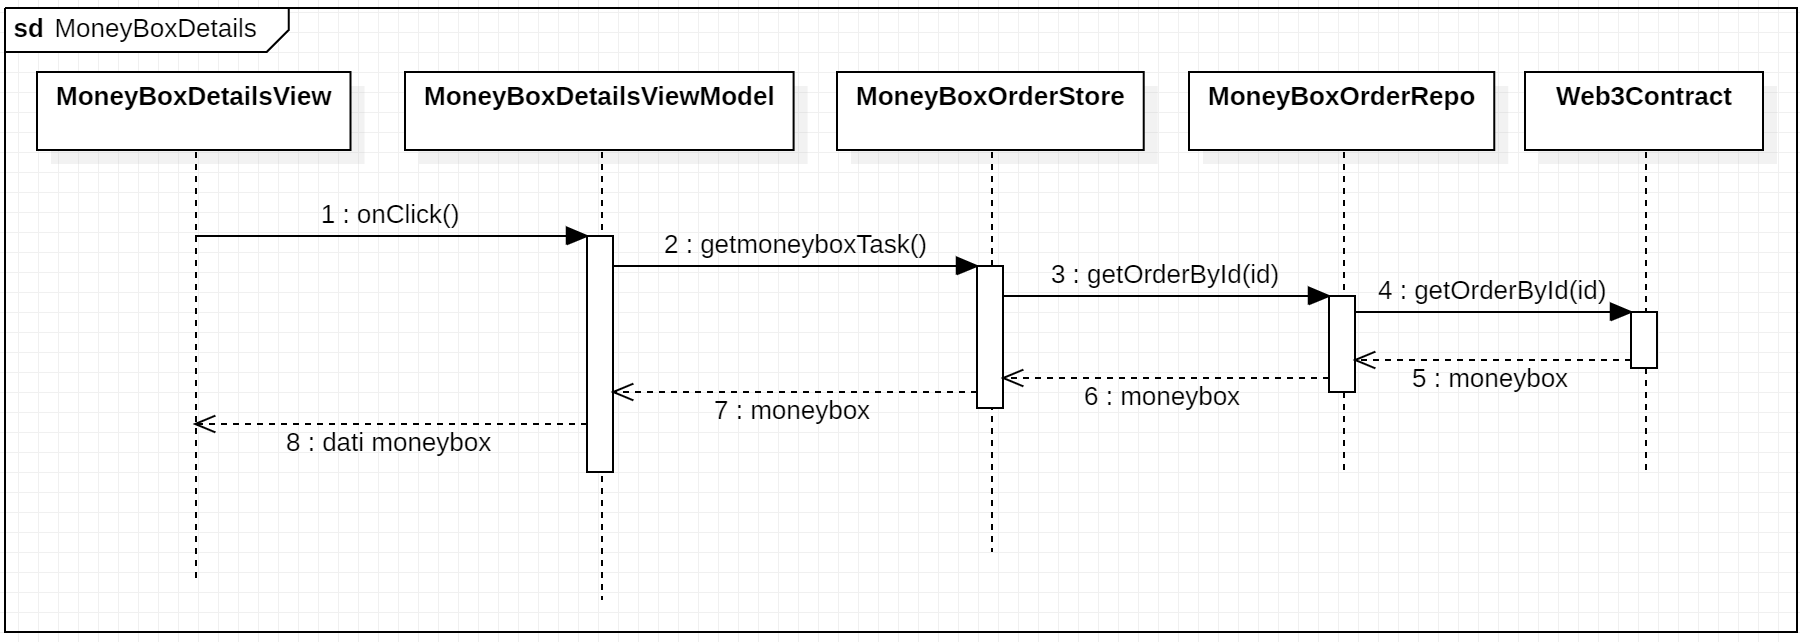
\includegraphics[width=\textwidth]{immagini/moneyboxdetails.png}
    \caption{Diagramma di sequenza della funzione di visualizzazione dei dettagli di una Moneybox}
    \end{center}
\end{figure}

\clearpage

\subsection{Design pattern}

Sono stati utilizzati due design pattern nello sviluppo dell'applicazione:
\begin{itemize}
    \item Singleton: è un design pattern che consente di garantire che una classe abbia una sola istanza, fornendo al contempo un punto di accesso globale a questa istanza;
    \item Repository Pattern: un repository incapsula un insieme di oggetti memorizzati nel database e le operazioni che possono essere eseguite su di essi.
\end{itemize}

Il design singleton è stato usato per avere un'unica fonte detentrice dello stato di ogni modello.
Il repository pattern ci ha permesso di racchiudere tutte le interazioni con sorgenti esterne in un oggetto unico, mantenendo la separazione tra implementazione e interfaccia.


%Descrivo qui se abbiamo utilizzato qualche design pattern in particolare